\chapter{VisualSfM}\label{sec:visualsfm}
%======================================================================================
%
\section*{Introdução}

VisualSfM é um {\it software} baseado em fotogrametria que faz todo o processo de reconstrução 3D de um objeto e que pode usá-lo por linha de comando ou então pela interface gráfica, que é ótima, por sinal. É altamente customizável, podendo utilizar o CUDA da NVIDIA ou OpenGL, especificar a lista de pares para correspondência de imagens, usar detectores de {\it features} próprios, velocidade da detecção de {\it features}, da reconstrução densa, dentre outros parâmetros. Ou seja, é um {\it software} robusto, que pode ser usado em Linux, Windows ou até mesmo Mac.

\section*{Procedimento}

Sua linha de reconstrução é parecida com o MVE \ref{sec:mve}, porém é mais intuitiva. Em sua interface, possui um Log de mensagens e erros que por ventura venham a acontecer e na parte de cima, alguns botões \ref{fig:pipelineVisualSfM}

\begin{figure}[!h]
	\centering

	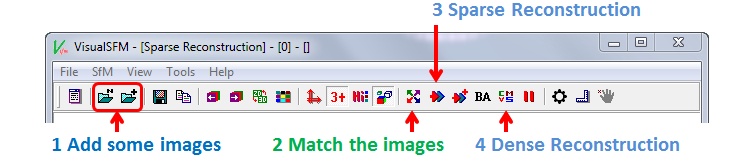
\includegraphics[width=1\linewidth]{figs/pipelinevisualsfm.png}
	\caption{%
	Botões na parte superior da interface gráfica, este seria o {\it pipeline} padrão de funcionamento do {\it software}.
	}\label{fig:pipelineVisualSfM}
\end{figure}

Como demonstrado na imagem \ref{fig:pipelineVisualSfM}, o funcionamento seria da seguinte forma:

\begin{itemize}
\item \textbf{1 - Adicionar algumas imagens.} Este é o primeiro passo, para começar uma reconstrução, primeiro adiciona-se imagens ao {\it software}, pode ser uma única foto, um conjunto de fotos, incrementar o conjunto já existente ou então abrir um arquivo de extensão .nvm, que é interpretado como uma reconstrução esparsa previamente feita.

\item \textbf{2 - Correspondência de imagens.} Agora, o {\it software} roda o algoritmo SIFT, realizando todas as correspondências entre os {\it features}.

\item \textbf{3 - Reconstrução esparsa.} Neste passo, o VisualSfM roda o algoritmo de reconstrução esparsa (PBA). %LEMBRAR QUAL É O ALGORITMO!!% 

esparsa em todos os {\it features} descobertos no passo passado.

\item \textbf{4 - Reconstrução densa.} Finalmente, acaba a reconstrução rodando o algoritmo CMVS/PMVS-2 embutido no próprio VisualSfM de reconstrução densa.
\end{itemize}

PBA -- {\it Parallel Banding Algorithm}

O PBA é um algoritmo implementado em GPU (Graphic Processor Unit) para computar a Distância de Transformação Euclidiana (EDT -- Euclidean Distance Transform) para uma imagem binária em 2D ou em dimensões superiores. Particionando a imagem em pequenas bandas para processar e posteriormente, juntando-as simultaneamente, o PBA calcula o EDT exato com ótimo trabalho linear total, alto nível de paralelismo e um bom padrão de acesso à memória. Este algoritmo foi um dos precursores em questão de tentar explorar o máximo desempenho da GPU no cálculo da EDT exata. 


% O PBA é divido em 3 fases:

% \begin{itemize}
% \item Band Sweeping
% \item Hierarchical Merging
% \item Block coloring
% \end{itemize}

% Band Sweeping

% In this phase, for each row, we want to compute the 1D Voronoi
% diagram using only those sites in the same row. A trivial approach
% would be to use a two-pass sweeping (left to right and then right to
% left sweeping), similar to SKW [Schneider et al. 2009]. This, however,
% restricts the parallelism to only one thread per row, potentially
% under-utilizing the GPU. One could also use a 1D JFA [Rong and
% Tan 2007] with better utilization of the GPU at the cost of higher
% total work. Another possibility would be to use a method similar
% to the work efficient parallel prefix sum [Harris et al. 2007]. This
% approach is too complicated as compared to our following simple,
% yet work and time efficient approach.
% Our approach extends the na¨ıve two-pass sweeping approach, with
% the introduction of bands to effectively increase the level of parallelism.
% First, we divide the input image into m1 vertical bands
% of equal size, and use one thread to handle one row in each band,
% performing the left-right sweeps. Next, for one site to propagate
% its information to a different band (on the same row), it has to be
% the closest site to the first or the last pixel of its band. As such, to
% combine the result of different bands into the needed answer, we
% first propagate the information among the first and the last pixels
% of all bands using a parallel prefix approach on these 2m1 pixels.
% With this, the first and the last pixel of each band have the correct
% information, whereas other pixels inside a band can then obtain the
% correct closest sites by updating (if needed) their current information
% with that of the first and the last pixel of their band. This can
% be done in parallel in constant time using N threads.

Hierarchical Merging




%FALAR SOBRE O ALGORITMO DE RECONSTRUCAO DENSA == PMVS-2/CMVS%



Além disso, o VisualSfM é capaz de mostrar a matriz de correspondência de {\it features}, número de {\it features}, rodar um {\it Bundle Adjustment}, usar um Level 0 no PVMS, alterar a memória de GPU usada na reconstrução, deletar uma reconstrução indesejável, alterar parâmetros e rodar novamente o passo a passo acima.